\documentclass[letterpaper,10pt,onecolumn]{article}
\usepackage[spanish]{babel}
\usepackage[utf8x]{inputenc}
\usepackage{amsfonts}
\usepackage{amsthm}
\usepackage{amsmath}
\usepackage{mathrsfs}
\usepackage{empheq}
\usepackage{enumitem}
\usepackage[pdftex]{color,graphicx}
\usepackage{hyperref}
\usepackage{listings}
\usepackage{calligra}
\usepackage{algpseudocode} 
\DeclareMathAlphabet{\mathcalligra}{T1}{calligra}{m}{n}
\DeclareFontShape{T1}{calligra}{m}{n}{<->s*[2.2]callig15}{}
\newcommand{\scripty}[1]{\ensuremath{\mathcalligra{#1}}}
\lstloadlanguages{[5.2]Mathematica}
\setlength{\oddsidemargin}{0cm}
\setlength{\textwidth}{490pt}
\setlength{\topmargin}{-40pt}
\addtolength{\hoffset}{-0.3cm}
\addtolength{\textheight}{4cm}

\begin{document}
\begin{center}



\includegraphics[width=490pt]{header.png}\\[0.5cm]

\textsc{\LARGE Taller 2 - F\'isica I (FISI-1018) - 2016-10}\\[0.5cm]

\textsc{\Large{Profesor: Jaime Forero}} \\[0.5cm]

\noindent\textsc{Ejercicios correspondiente a la clase complementaria
  de la semana del 1 de Febrero del 2016.}\\[0.5cm]
\end{center}

\noindent\textsc{Nota:} 
Los primeros tres ejercicios deben ser
entregados {\bf al comienzo} de la clase complementaria. Los \'ultimos
cuatro deben ser trabajados {\bf durante} la complementaria. 

La numeraci\'on
hace referencia al texto gu\'ia: \textit{F\'isica Universitaria Volumen
  1 (Sears-Semansky)}, decimotercera edici\'on, Pearson.

\begin{enumerate}
% aqui vienen los tres ejercicios "faciles"

\item
\begin{enumerate}
\item Se tienen dos vectores $\vec{A}=(2\hat{\i}-3\hat{\j}+7\hat{k})$ y $\vec{B}=(5\hat{\i}+\hat{\j}+2\hat{k})$. Encuentre: $\vec{A}+\vec{B}$ y $\vec{A}-\vec{B}$. 
\item Muestre que si un vector $\vec{A}$ es perpendicular a $\vec{B}$, entonces $|\vec{A}+\vec{B}|=|\vec{A}-\vec{B}|$. 
\end{enumerate} %propuesto por Miguel

\item Ejercicio 1.66 (Equilibrio de fuerzas). % propuesto por Jaime

\item El salón de clases de Laura y Camila mide 7 m por 7 m; en la esquina A se encuentran las dos estudiantes. Laura caminará hacia la puerta, ubicada en la esquina C, por la diagonal del salón, mientras Camila se dirigirá primero a la esquina O y de allí irá directo a la puerta. Si Laura camina hacia la puerta a una velocidad de 1.1 m/s y Camila tarda 5 segundos en llegar hasta la esquina O, ¿cuál debe ser la velocidad promedio de Camila en el trayecto O-A para que llegue a la puerta al mismo tiempo que Laura?
\begin{figure}[h]
  \centering
  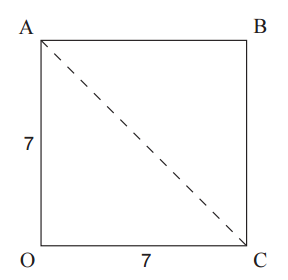
\includegraphics[width=0.35\textwidth]{salon}
  \caption{Salón de Laura y Camila} \label{f:salon}
\end{figure} %propuesto por Juan Carlos

% aqui vienen los cuatro ejercicios "dificiles"
\item Ejercicio 2.42 (Ladrillo cayendo de un edificio). % propuesto por Jaime
\item Ejercicio 2.54 (Salto volador de una pulga). % propuesto Jaime

\item Un pirata ha enterrado su tesosro en una isla remota, en la cual sólo hay 5 palmeras localizadas en los puntos: (30 m, -20 m), (60 m, 80 m), (-10 m, -10 m), (40 m, -30 m) y (-70, 60 m) con respecto a cierto origen. Las instrucciones del mapa, que usted ha encontrado, senalan que comenzando en la palmera A camine directo hacia la palmera B, deteniendosé en la mitad del trayecto. Desde allí dirigase hacia la palmera C, pero recorra sólo un tercio de la distancia. Desde este nuevo punto, dirígase hacia la palmera D pero sólo moviendose un cuarto de la distancia. Finalmente, desde allí camine hacia la palmera E y detengasé al reciorrer un quinto de la distancia. 
\begin{enumerate}
\item ¿En qué coordenadas se encuentra el tesoro?, asuma que el orden de las coordenadas de las palmeras corresponde a A,B,C,D y E.
\item Suponga que usted desconoce cuál es cada una de las palemras, es decir, no sabe donde comenzar ni hacia donde seguir  en cada paso. Escoja un orden diferente para las palmeras e indiqué la ``nueva'' ubicación del tesoro. ¿La respuesta es independiente del orden escogido? Explique
\end{enumerate}  %propuesto por Juan Carlos

\item
Durante un accidente automovilístico, las bolsas de aire del vehículo se inflan y desaceleran a los pasajeros más suavemente que si golpearan el parabrisas o el volante directamente. De acuerdo con las normas de seguridad, las bolsas producen una aceleración máxima de $60g$ que dura solo $36$ms. ¿Que distancia recorre una persona antes de detenerse completamente en $36$ms con aceleración constante de $60 g$, donde $g$ es la magnitud de la aceleraci\'on de la gravedad?  
 %propuesto por Miguel

\end{enumerate}

\end{document}
